\chapter{THỰC NGHIỆM VÀ ĐÁNH GIÁ}

\section{Thiết lập thực nghiệm đa phương thức}
Thực nghiệm được tổ chức theo hai nhánh chính: nhánh phân tích văn bản bằng PhoBERT và nhánh phát hiện hình ảnh bằng YOLO. Hai nhánh này đánh giá các dạng tín hiệu khác nhau và cùng đóng góp vào hệ thống tổng. Kết quả của từng nhánh không được diễn giải như kết luận pháp lý độc lập, mà là bằng chứng hỗ trợ tầng hợp nhất rủi ro.

Nhánh PhoBERT sử dụng \texttt{PhoBERT-base-v2} được fine-tune cho bài toán phân loại đa nhãn bằng lớp phân loại chuỗi của Transformers. Nhánh YOLO sử dụng YOLO11m pretrained weights, huấn luyện trên dataset Roboflow \texttt{doctor-and-medical} version 7, export theo YOLO format và đánh giá bằng checkpoint \texttt{best.pt}.

\section{Dữ liệu và chỉ số đánh giá}
\subsection{Dữ liệu văn bản}
\begin{table}[H]
\centering
\caption{Thống kê số lượng mẫu văn bản theo tập dữ liệu}
\label{tab:text_split_stats}
\begin{tabular}{|l|r|r|}
\hline
\textbf{Tập dữ liệu} & \textbf{Số mẫu} & \textbf{Tỷ lệ} \\
\hline
Train & 2289 & 82.1\% \\ \hline
Validation & 249 & 8.9\% \\ \hline
Test & 249 & 8.9\% \\ \hline
\end{tabular}
\end{table}

Tổng số mẫu văn bản sau khi chia tập là 2787. Quá trình chia dữ liệu theo \texttt{post\_id} không phát hiện nhóm leakage giữa các tập, với \texttt{Post\_id leakage groups} bằng 0.

\begin{table}[H]
\centering
\caption{Thống kê phân phối nhãn văn bản}
\label{tab:text_label_distribution}
\begin{tabularx}{\textwidth}{|L{0.35\textwidth}|r|r|Y|}
\hline
\textbf{Nhãn} & \textbf{Số mẫu dương} & \textbf{Tỷ lệ} & \textbf{Nhận xét} \\
\hline
\texttt{IS\_ADS} & 1327 & 47.6\% & Nhãn quảng cáo tổng quát có số mẫu dương lớn nhất. \\ \hline
\texttt{EFFICACY\_CLAIM} & 1233 & 44.2\% & Nhãn công dụng xuất hiện phổ biến trong dữ liệu. \\ \hline
\texttt{CURE\_CLAIM} & 397 & 14.2\% & Nhãn chữa bệnh có số mẫu trung bình. \\ \hline
\texttt{AUTHORITY\_REFERENCE} & 658 & 23.6\% & Nhãn tham chiếu uy tín xuất hiện tương đối nhiều. \\ \hline
\texttt{TESTIMONIAL} & 117 & 4.2\% & Nhãn hiếm, cần theo dõi khi đánh giá macro F1. \\ \hline
\texttt{FEAR\_URGENCY} & 124 & 4.4\% & Nhãn hiếm, dễ bị ảnh hưởng bởi mất cân bằng dữ liệu. \\ \hline
\texttt{PRICE\_PROMOTION} & 365 & 13.1\% & Nhãn khuyến mãi có số mẫu trung bình. \\ \hline
\end{tabularx}
\end{table}

\subsection{Dữ liệu hình ảnh}
Test set của nhánh YOLO gồm 160 ảnh, 256 object instances và 1 ảnh nền. Mô hình đánh giá là YOLO11m với 20,033,887 tham số và 67.7 GFLOPs. Các lớp được đánh giá gồm \texttt{Lab-coat}, \texttt{logo}, \texttt{stethoscope} và \texttt{Shirt}.

\subsection{Chỉ số đánh giá}
Với nhánh PhoBERT, các chỉ số gồm exact match accuracy, precision, recall, macro F1 và micro F1. Macro F1 phản ánh hiệu quả trên từng nhãn theo trung bình không trọng số, còn micro F1 phản ánh hiệu quả tổng thể trên toàn bộ dự đoán.

Các chỉ số Precision, Recall và F1 được tính từ số lượng true positive (TP), false positive (FP) và false negative (FN):
\[
\mathrm{Precision} = \frac{TP}{TP + FP},
\quad
\mathrm{Recall} = \frac{TP}{TP + FN},
\quad
F1 = \frac{2 \times \mathrm{Precision} \times \mathrm{Recall}}
{\mathrm{Precision} + \mathrm{Recall}}
\]
Với bài toán đa nhãn, exact match accuracy yêu cầu toàn bộ vector nhãn dự đoán phải trùng với vector nhãn thật:
\[
\mathrm{ExactMatch}
= \frac{1}{N}\sum_{j=1}^{N}
\mathbf{1}\left(\hat{\mathbf{y}}^{(j)} = \mathbf{y}^{(j)}\right)
\]
Trong đó \(N\) là số mẫu, \(\hat{\mathbf{y}}^{(j)}\) là vector nhãn dự đoán và \(\mathbf{y}^{(j)}\) là vector nhãn thật của mẫu thứ \(j\).

Với nhánh YOLO, Precision cho biết tỷ lệ dự đoán đúng trong các object được mô hình phát hiện, Recall cho biết tỷ lệ object thật được phát hiện, mAP50 là mean average precision tại ngưỡng IoU 0.5, mAP50-95 là mAP trung bình trên nhiều ngưỡng IoU từ 0.5 đến 0.95, còn mAP75 là mAP tại ngưỡng IoU 0.75. mAP50-95 khắt khe hơn vì đánh giá cả chất lượng định vị bounding box ở nhiều mức IoU.

Average Precision (AP) của một lớp được hiểu là diện tích dưới đường cong Precision--Recall:
\[
AP_c = \int_{0}^{1} P_c(r)\,dr
\]
mAP tại một ngưỡng IoU \(t\) là trung bình AP trên \(C\) lớp:
\[
\mathrm{mAP}@t = \frac{1}{C}\sum_{c=1}^{C} AP_c(t)
\]
Với mAP50-95, kết quả được lấy trung bình trên các ngưỡng IoU từ 0.50 đến 0.95 với bước 0.05:
\[
\mathrm{mAP}_{50:95}
= \frac{1}{10}\sum_{t \in \{0.50,0.55,\ldots,0.95\}}
\mathrm{mAP}@t
\]

\section{Kết quả nhánh văn bản PhoBERT}
\subsection{Threshold và kết quả tổng quan}
\begin{table}[H]
\centering
\caption{Threshold cuối cùng dùng để đánh giá validation/test}
\label{tab:phobert_thresholds}
\begin{tabular}{|l|r|}
\hline
\textbf{Nhãn} & \textbf{Threshold} \\
\hline
\texttt{EFFICACY\_CLAIM} & 0.57 \\ \hline
\texttt{CURE\_CLAIM} & 0.73 \\ \hline
\texttt{AUTHORITY\_REFERENCE} & 0.59 \\ \hline
\texttt{TESTIMONIAL} & 0.65 \\ \hline
\texttt{FEAR\_URGENCY} & 0.27 \\ \hline
\texttt{PRICE\_PROMOTION} & 0.60 \\ \hline
\texttt{IS\_ADS} & 0.65 \\ \hline
\end{tabular}
\end{table}

\begin{table}[H]
\centering
\caption{Kết quả tổng quan của PhoBERT trên validation và test}
\label{tab:phobert_overall_results}
\begin{tabular}{|l|r|r|r|r|r|}
\hline
\textbf{Tập} & \textbf{Exact match} & \textbf{Macro F1} & \textbf{Micro F1} & \textbf{Macro P} & \textbf{Macro R} \\
\hline
Validation & 0.6747 & 0.7522 & 0.8468 & 0.7191 & 0.8304 \\ \hline
Test & 0.6546 & 0.6413 & 0.8183 & 0.6115 & 0.6790 \\ \hline
\end{tabular}
\end{table}

\subsection{Kết quả theo nhãn}
\begin{table}[H]
\centering
\caption{Kết quả PhoBERT theo từng nhãn trên tập test}
\label{tab:phobert_per_label_results}
\begin{tabularx}{\textwidth}{|L{0.30\textwidth}|r|r|r|r|Y|}
\hline
\textbf{Nhãn} & \textbf{P} & \textbf{R} & \textbf{F1} & \textbf{Support} & \textbf{Nhận xét} \\
\hline
\texttt{EFFICACY\_CLAIM} & 0.7177 & 0.8812 & 0.7911 & 101 & Recall cao, phù hợp với mục tiêu phát hiện claim công dụng. \\ \hline
\texttt{CURE\_CLAIM} & 0.8056 & 0.8286 & 0.8169 & 35 & Kết quả tương đối ổn định dù support thấp hơn nhãn công dụng. \\ \hline
\texttt{AUTHORITY\_REFERENCE} & 0.7808 & 0.9344 & 0.8507 & 61 & Nhãn đạt F1 cao trong các nhóm nội dung rủi ro. \\ \hline
\texttt{TESTIMONIAL} & 0.0000 & 0.0000 & 0.0000 & 4 & Chưa học tốt do số mẫu dương rất ít. \\ \hline
\texttt{FEAR\_URGENCY} & 0.2857 & 0.4000 & 0.3333 & 5 & Kết quả còn hạn chế do nhãn hiếm và biểu đạt đa dạng. \\ \hline
\texttt{PRICE\_PROMOTION} & 0.8333 & 0.7812 & 0.8065 & 32 & Tín hiệu khuyến mãi tương đối rõ, F1 đạt mức tốt. \\ \hline
\texttt{IS\_ADS} & 0.8571 & 0.9273 & 0.8908 & 110 & Nhãn quảng cáo tổng quát đạt kết quả tốt. \\ \hline
\end{tabularx}
\end{table}

Trên tập test, PhoBERT đạt micro F1 là 0.8183 và macro F1 là 0.6413. Chênh lệch giữa micro F1 và macro F1 cho thấy mô hình hoạt động tốt hơn trên các nhãn phổ biến, trong khi hiệu quả giảm ở các nhãn hiếm như \texttt{TESTIMONIAL} và \texttt{FEAR\_URGENCY}. Kết quả này phù hợp với đặc điểm dữ liệu mất cân bằng và cho thấy cần tiếp tục mở rộng các nhóm nhãn hiếm.

\section{Kết quả nhánh hình ảnh YOLO}
\subsection{Kết quả tổng thể}
\begin{table}[H]
\centering
\caption{Kết quả tổng thể của YOLO11m trên test set}
\label{tab:yolo_overall_metrics}
\begin{tabularx}{\textwidth}{|L{0.38\textwidth}|Y|}
\hline
\textbf{Chỉ số} & \textbf{Giá trị} \\
\hline
Test images & 160 \\ \hline
Object instances & 256 \\ \hline
Background images & 1 \\ \hline
Parameters & 20,033,887 \\ \hline
GFLOPs & 67.7 \\ \hline
Precision & 0.898 \\ \hline
Recall & 0.818 \\ \hline
mAP50 & 0.872 \\ \hline
mAP75 & 0.830 \\ \hline
mAP50-95 & 0.733 \\ \hline
Preprocess speed & 5.7 ms/image \\ \hline
Inference speed & 27.6 ms/image \\ \hline
Postprocess speed & 1.5 ms/image \\ \hline
\end{tabularx}
\end{table}

Kết quả tổng thể cho thấy mô hình YOLO11m bước đầu phát hiện tương đối tốt các đối tượng hình ảnh liên quan đến bối cảnh y tế hoặc mạo danh uy tín trong quảng cáo. mAP50 đạt 0.872 và mAP50-95 đạt 0.733, cho thấy mô hình có khả năng phát hiện object ở mức khá, đồng thời vẫn còn dư địa cải thiện về định vị bounding box ở các ngưỡng IoU khắt khe hơn.

\subsection{Kết quả theo từng lớp}
\begin{table}[H]
\centering
\caption{Kết quả YOLO11m theo từng lớp trên test set}
\label{tab:yolo_class_metrics}
\begin{tabularx}{\textwidth}{|L{0.20\textwidth}|r|r|r|r|r|Y|}
\hline
\textbf{Lớp} & \textbf{Images} & \textbf{Inst.} & \textbf{P} & \textbf{R} & \textbf{mAP50} & \textbf{Nhận xét} \\
\hline
\texttt{Lab-coat} & 47 & 52 & 0.858 & 0.808 & 0.870 & Nhận diện khá tốt áo blouse trắng, là lớp mục tiêu chính. \\ \hline
\texttt{Shirt} & 54 & 96 & 0.815 & 0.635 & 0.730 & Lớp phụ/đối chứng, recall thấp hơn nhưng không phải lớp vi phạm chính. \\ \hline
\texttt{logo} & 80 & 97 & 0.927 & 0.921 & 0.948 & Lớp có kết quả tốt nhất, quan trọng cho nhóm nguy cơ mạo danh/lợi dụng uy tín. \\ \hline
\texttt{stethoscope} & 10 & 11 & 0.992 & 0.909 & 0.939 & Kết quả cao nhưng số mẫu còn ít, cần thận trọng khi kết luận độ ổn định. \\ \hline
\end{tabularx}
\end{table}

\begin{table}[H]
\centering
\caption{mAP50-95 theo từng lớp của YOLO11m}
\label{tab:yolo_map5095_by_class}
\begin{tabular}{|l|r|}
\hline
\textbf{Lớp} & \textbf{mAP50-95} \\
\hline
\texttt{Lab-coat} & 0.749 \\ \hline
\texttt{Shirt} & 0.602 \\ \hline
\texttt{logo} & 0.835 \\ \hline
\texttt{stethoscope} & 0.747 \\ \hline
\end{tabular}
\end{table}

Nếu chỉ xét ba lớp mục tiêu chính \texttt{Lab-coat}, \texttt{logo} và \texttt{stethoscope}, kết quả trung bình xấp xỉ đạt Precision 0.926, Recall 0.879, mAP50 0.919 và mAP50-95 0.777. Điều này cho thấy các lớp phục vụ trực tiếp cho phát hiện dấu hiệu hình ảnh rủi ro có kết quả tốt hơn trung bình chung khi không tính lớp phụ \texttt{Shirt}.

\subsection{Trực quan hóa kết quả YOLO}
\begin{figure}[H]
\centering
\begin{subfigure}{0.48\textwidth}
    \centering
    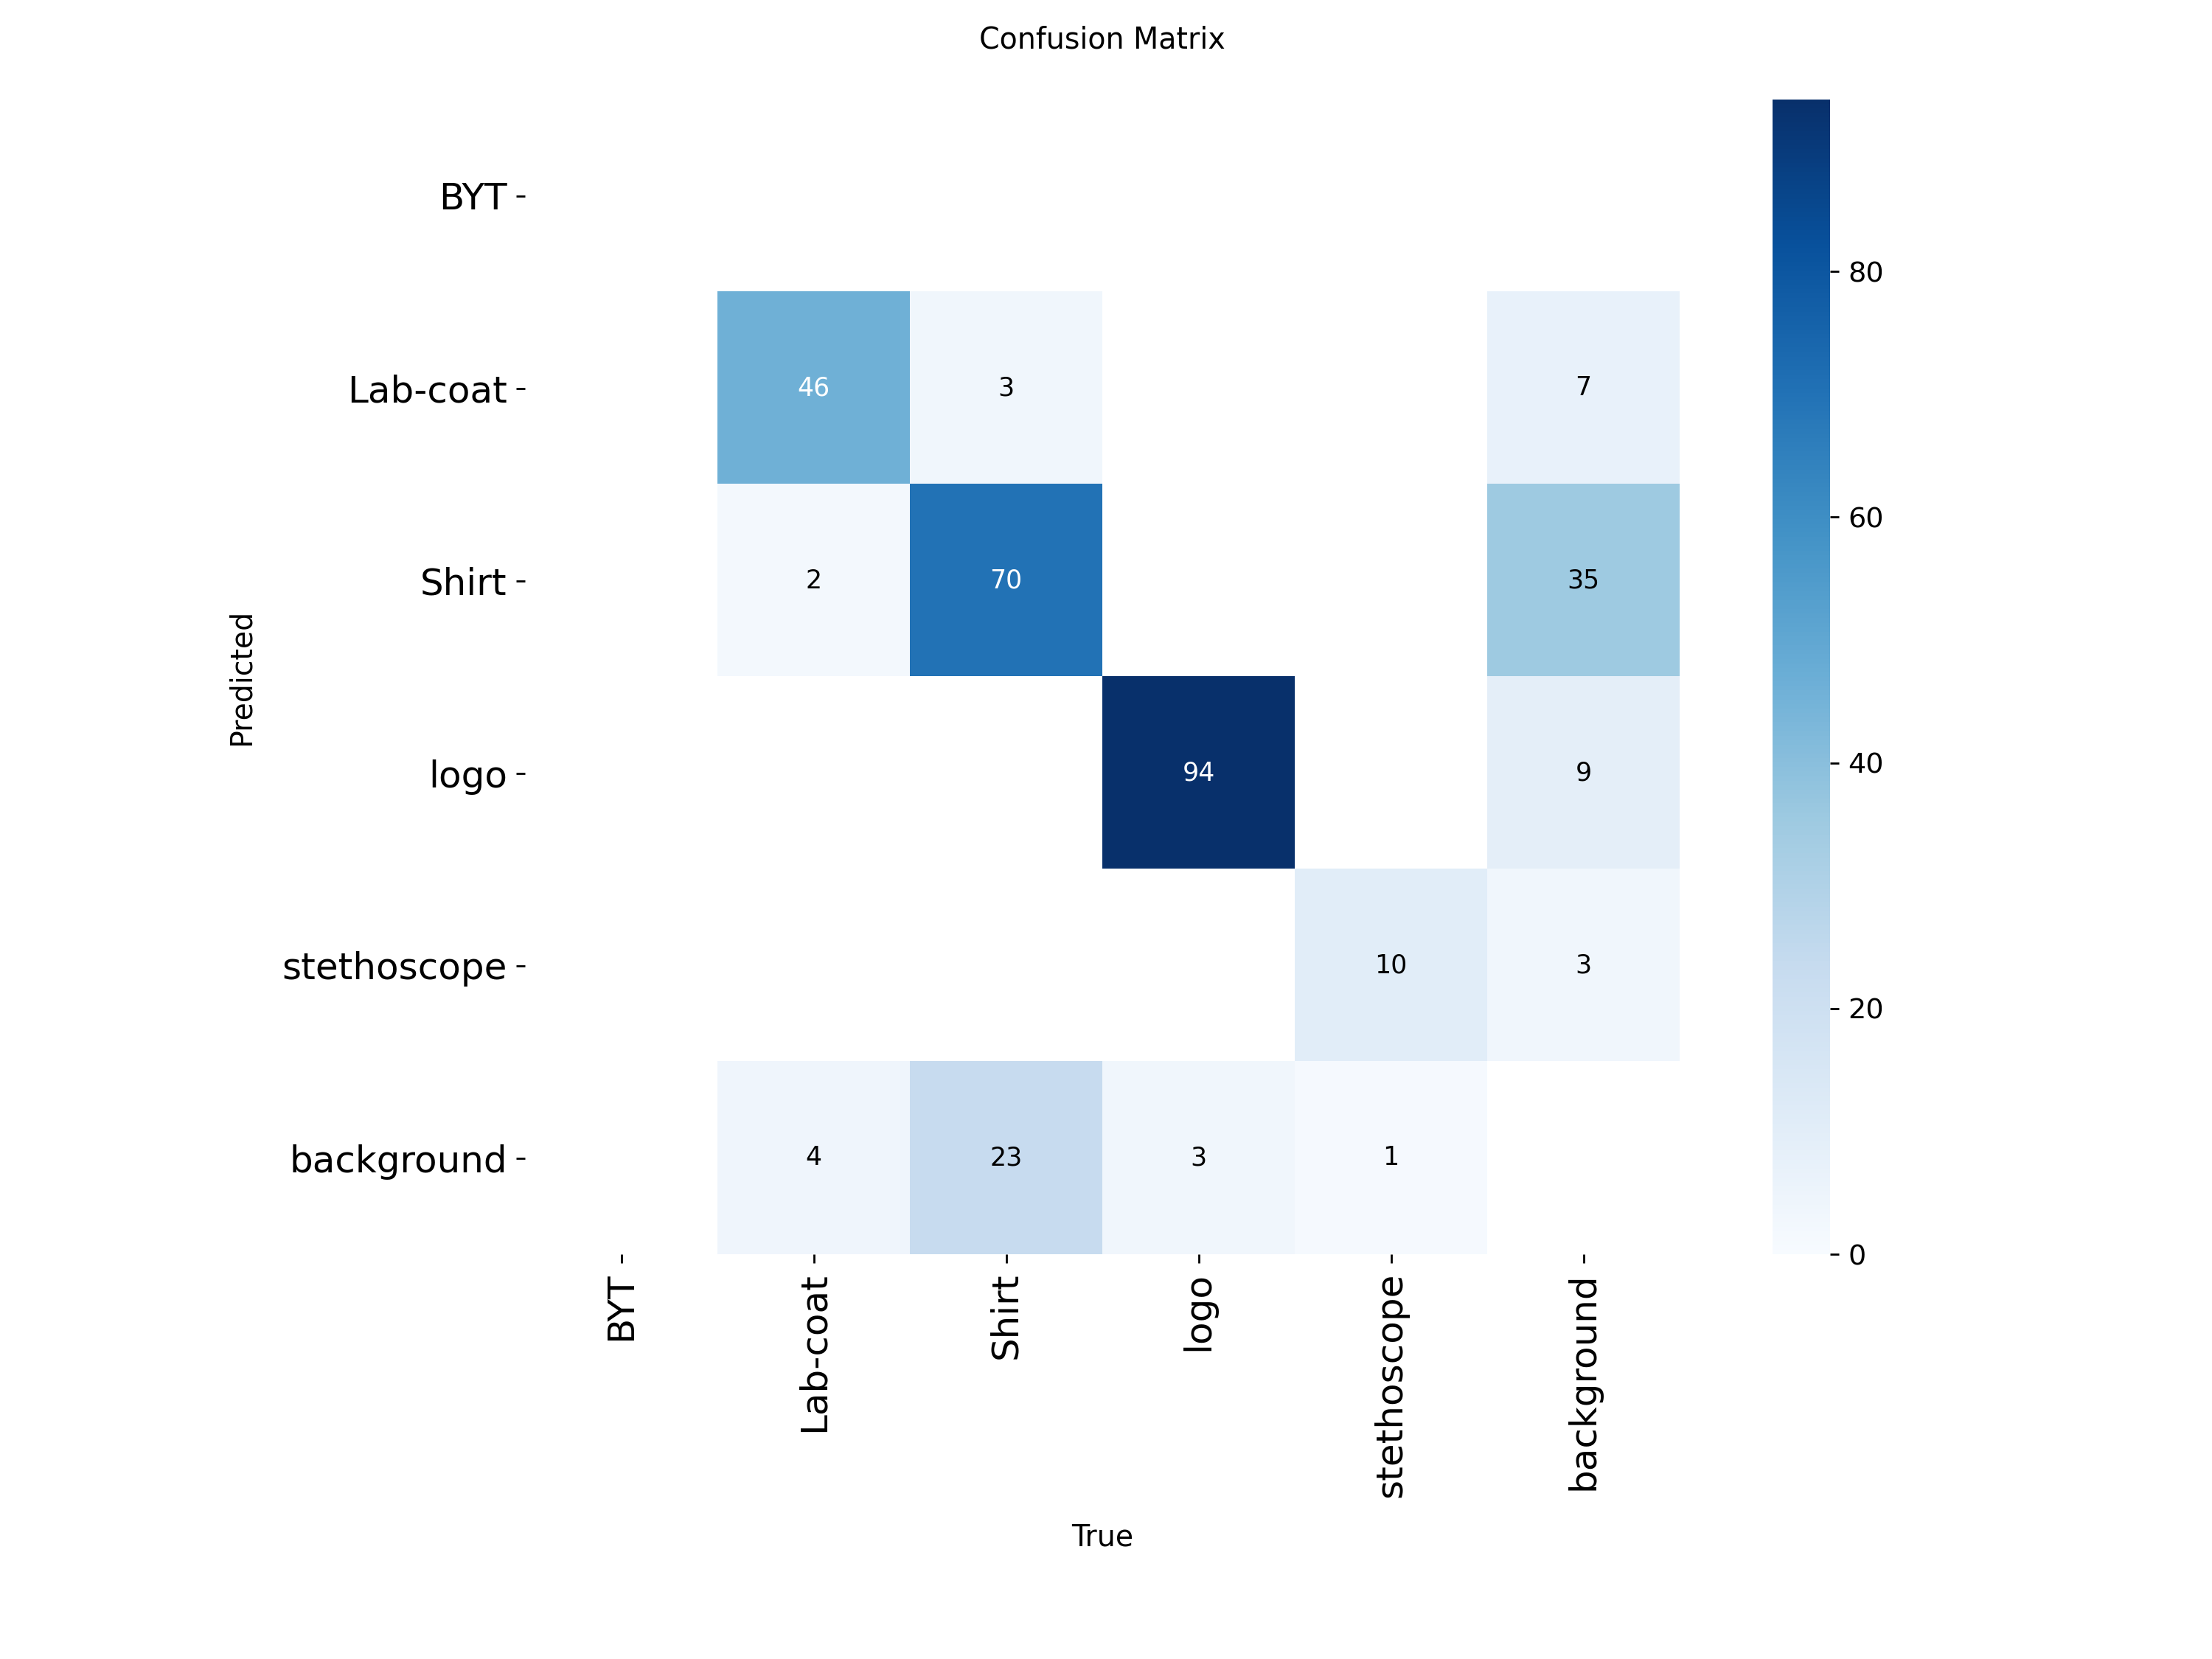
\includegraphics[width=\linewidth]{images/confusion_matrix.png}
    \caption{Ma trận nhầm lẫn theo số lượng}
    \label{fig:yolo_confusion_matrix}
\end{subfigure}
\hfill
\begin{subfigure}{0.48\textwidth}
    \centering
    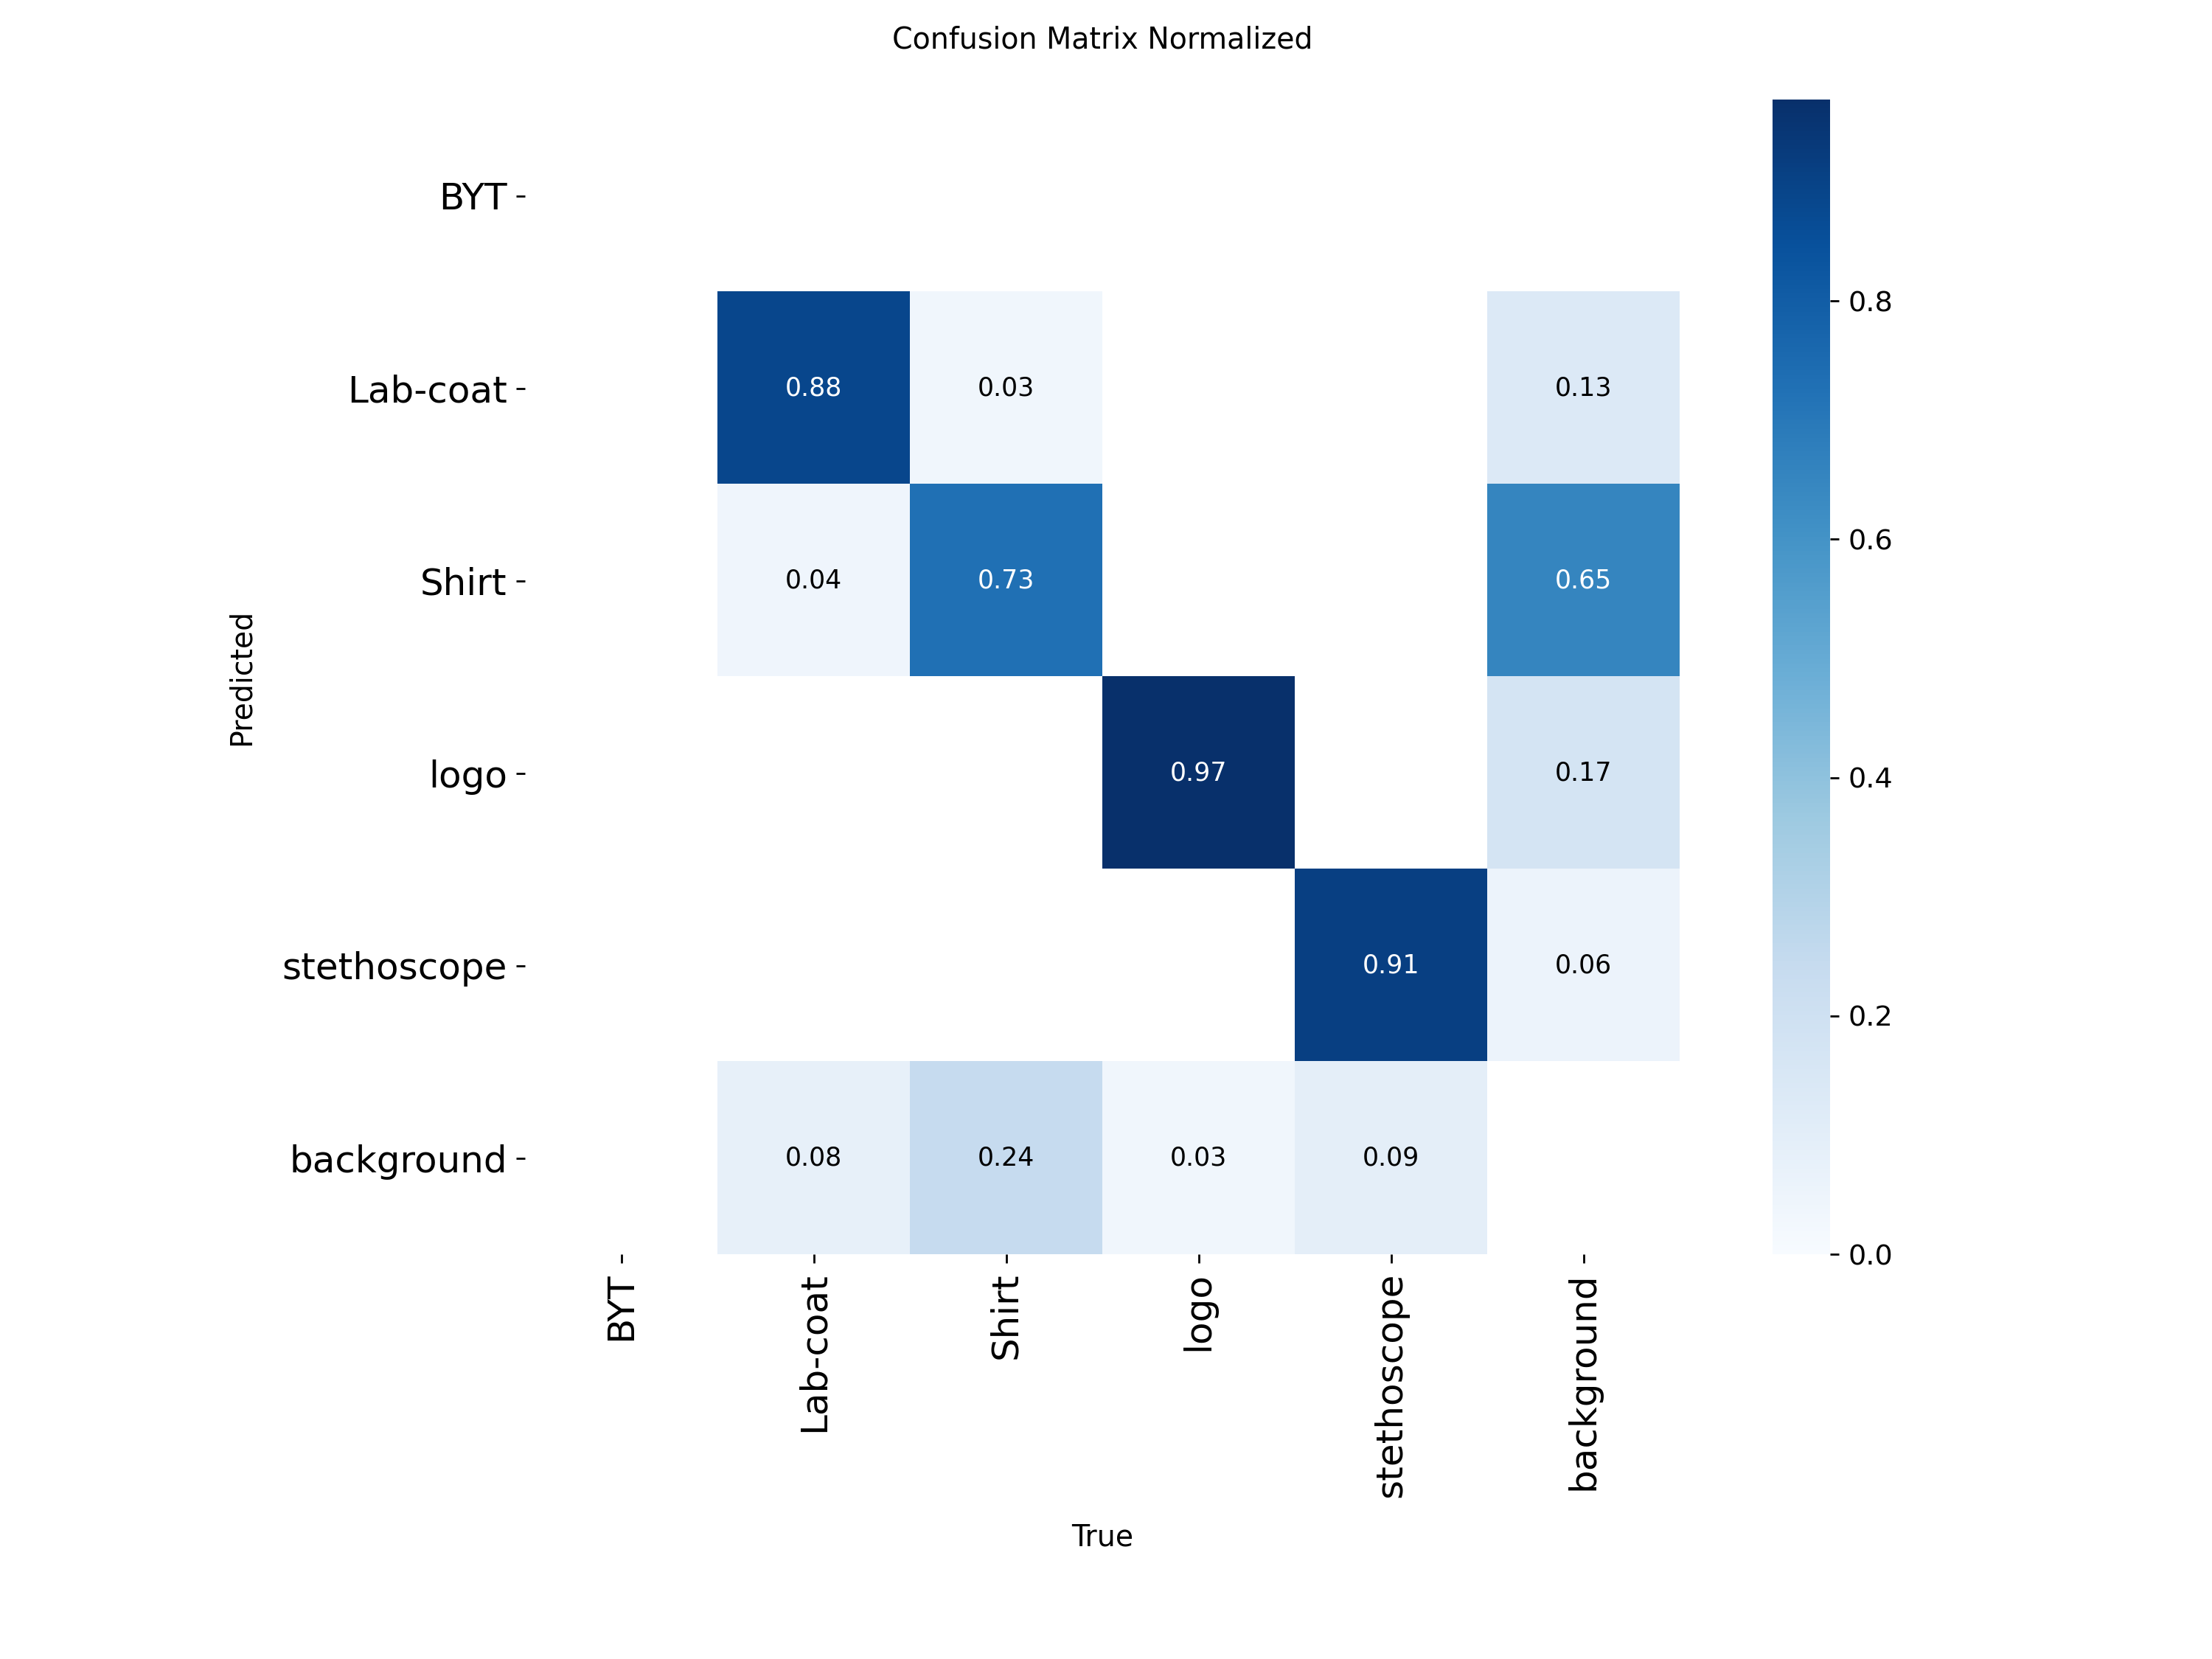
\includegraphics[width=\linewidth]{images/confusion_matrix_normalized.png}
    \caption{Ma trận nhầm lẫn chuẩn hóa}
    \label{fig:yolo_confusion_matrix_normalized}
\end{subfigure}
\caption{Ma trận nhầm lẫn của YOLO11m trên tập test}
\label{fig:yolo_confusion_matrices}
\end{figure}

Hai ma trận nhầm lẫn trong Hình~\ref{fig:yolo_confusion_matrices} hỗ trợ phân tích các trường hợp mô hình nhận diện sai hoặc bỏ sót object theo từng lớp. Ma trận chuẩn hóa giúp quan sát tỷ lệ lỗi giữa các lớp có số lượng mẫu khác nhau, trong khi ma trận theo số lượng cho thấy quy mô thực tế của từng nhóm lỗi.

\begin{figure}[H]
\centering
\begin{subfigure}{0.48\textwidth}
    \centering
    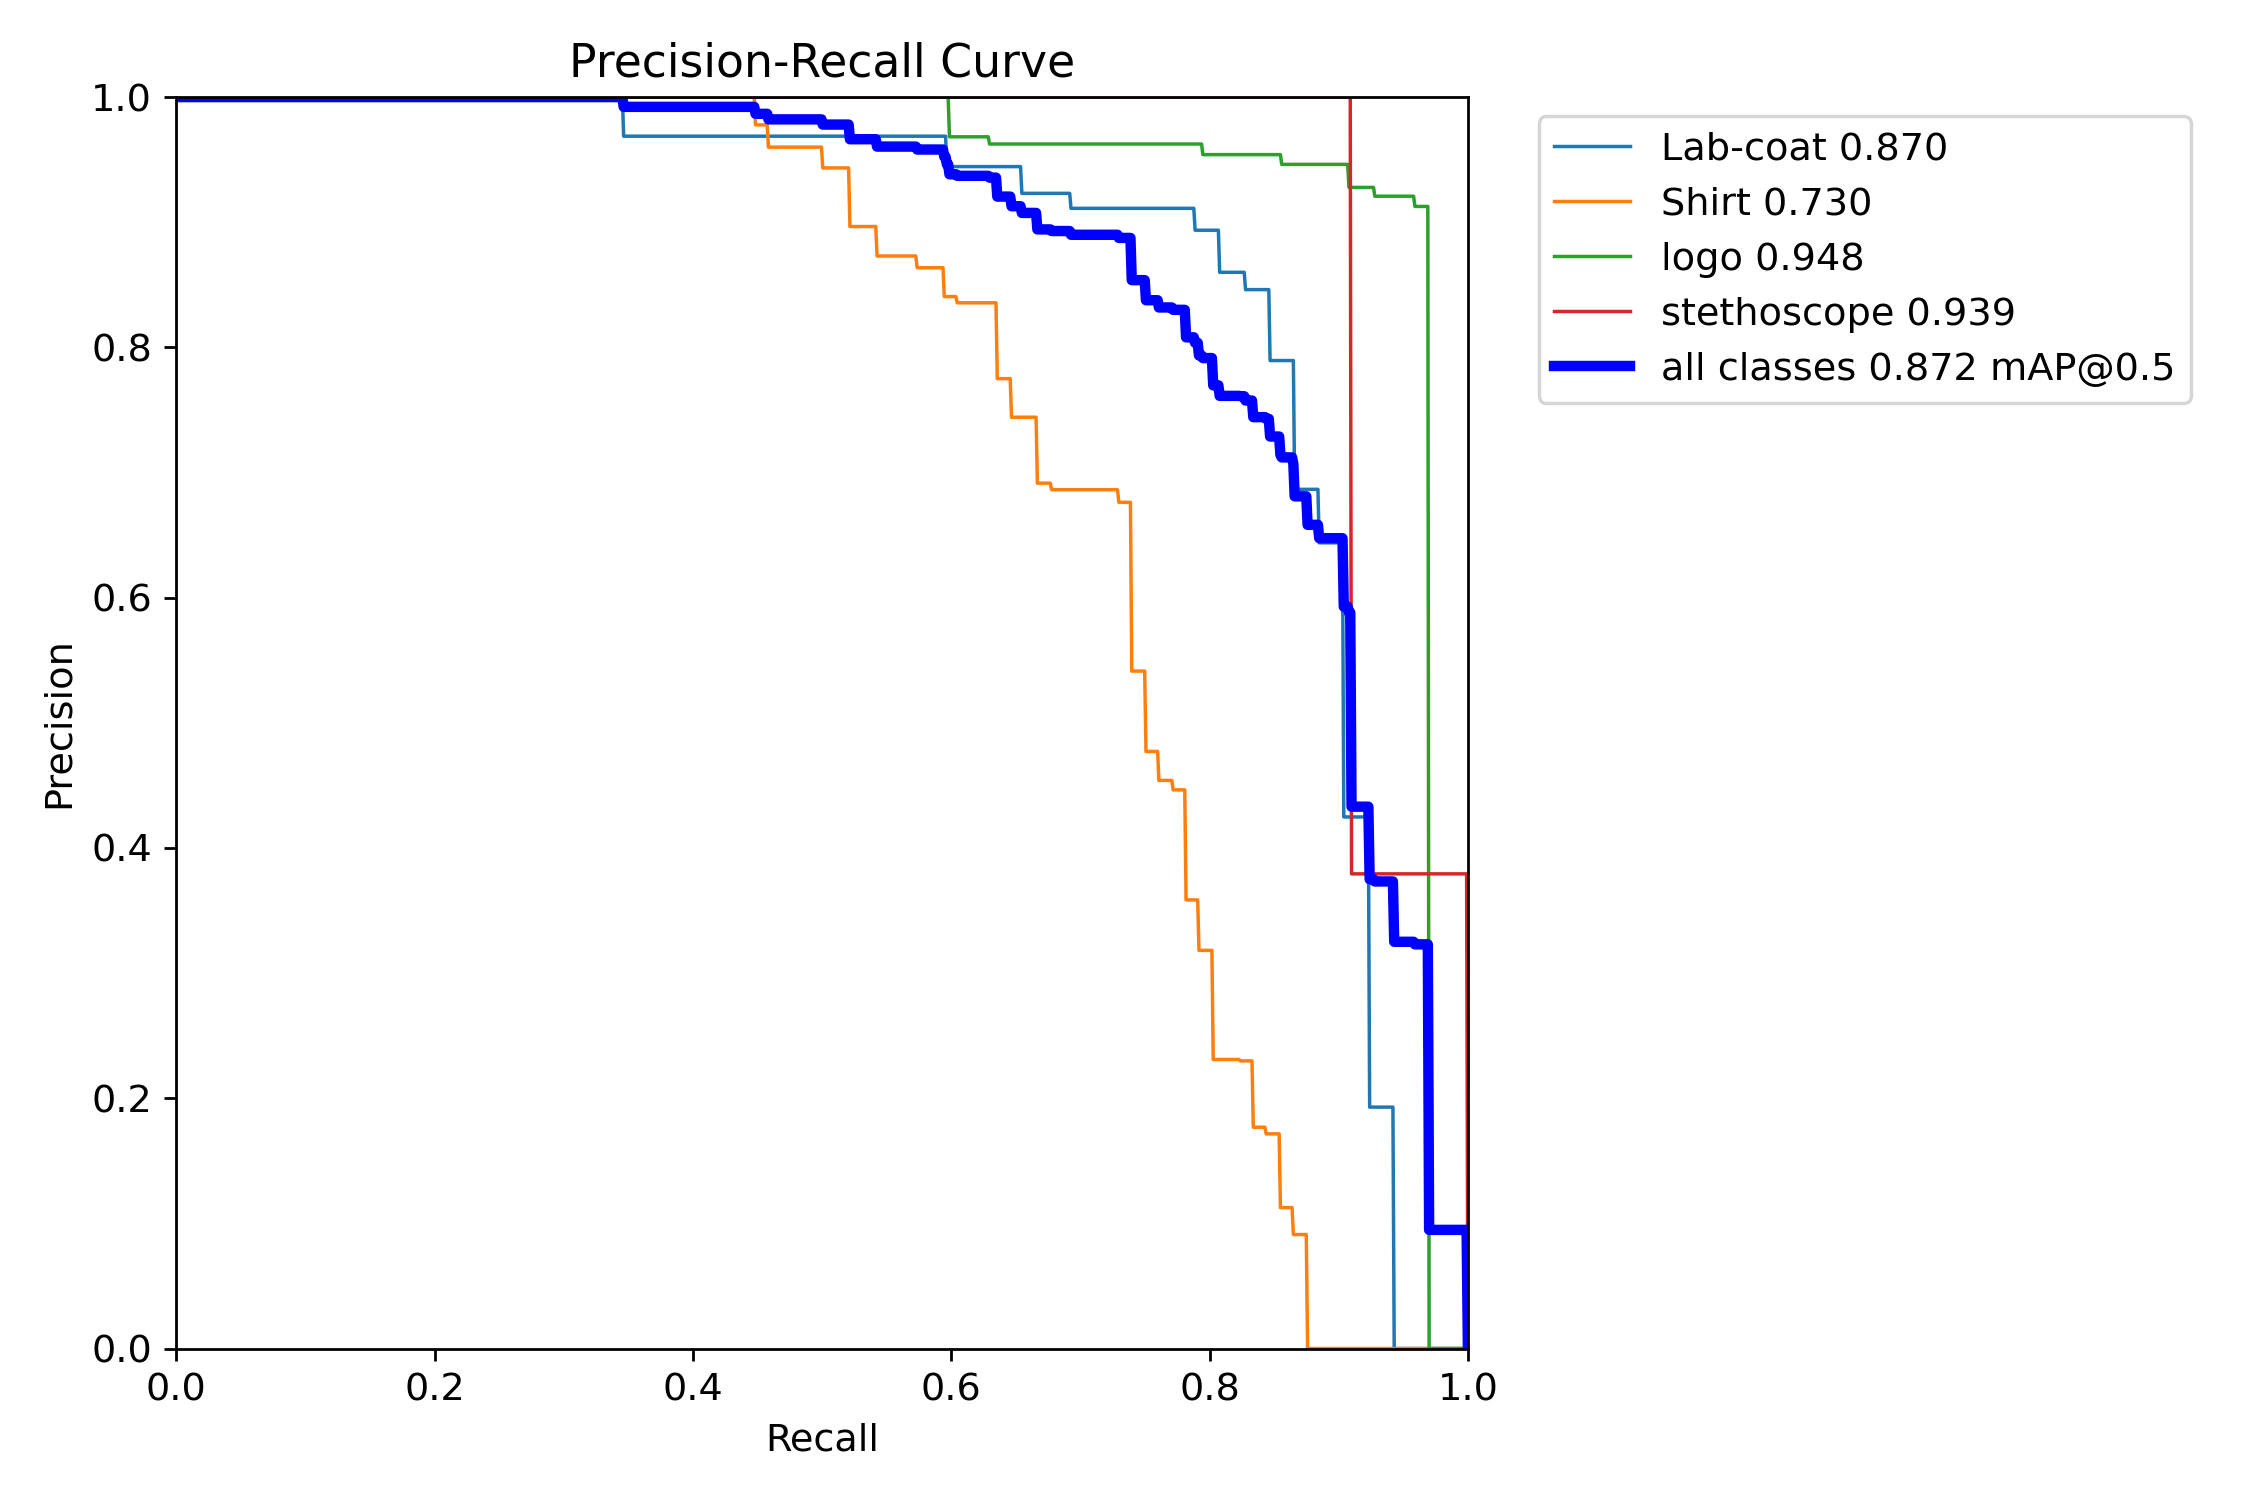
\includegraphics[width=\linewidth]{images/BoxPR_curve.png}
    \caption{Đường cong Precision--Recall}
    \label{fig:yolo_box_pr_curve}
\end{subfigure}
\hfill
\begin{subfigure}{0.48\textwidth}
    \centering
    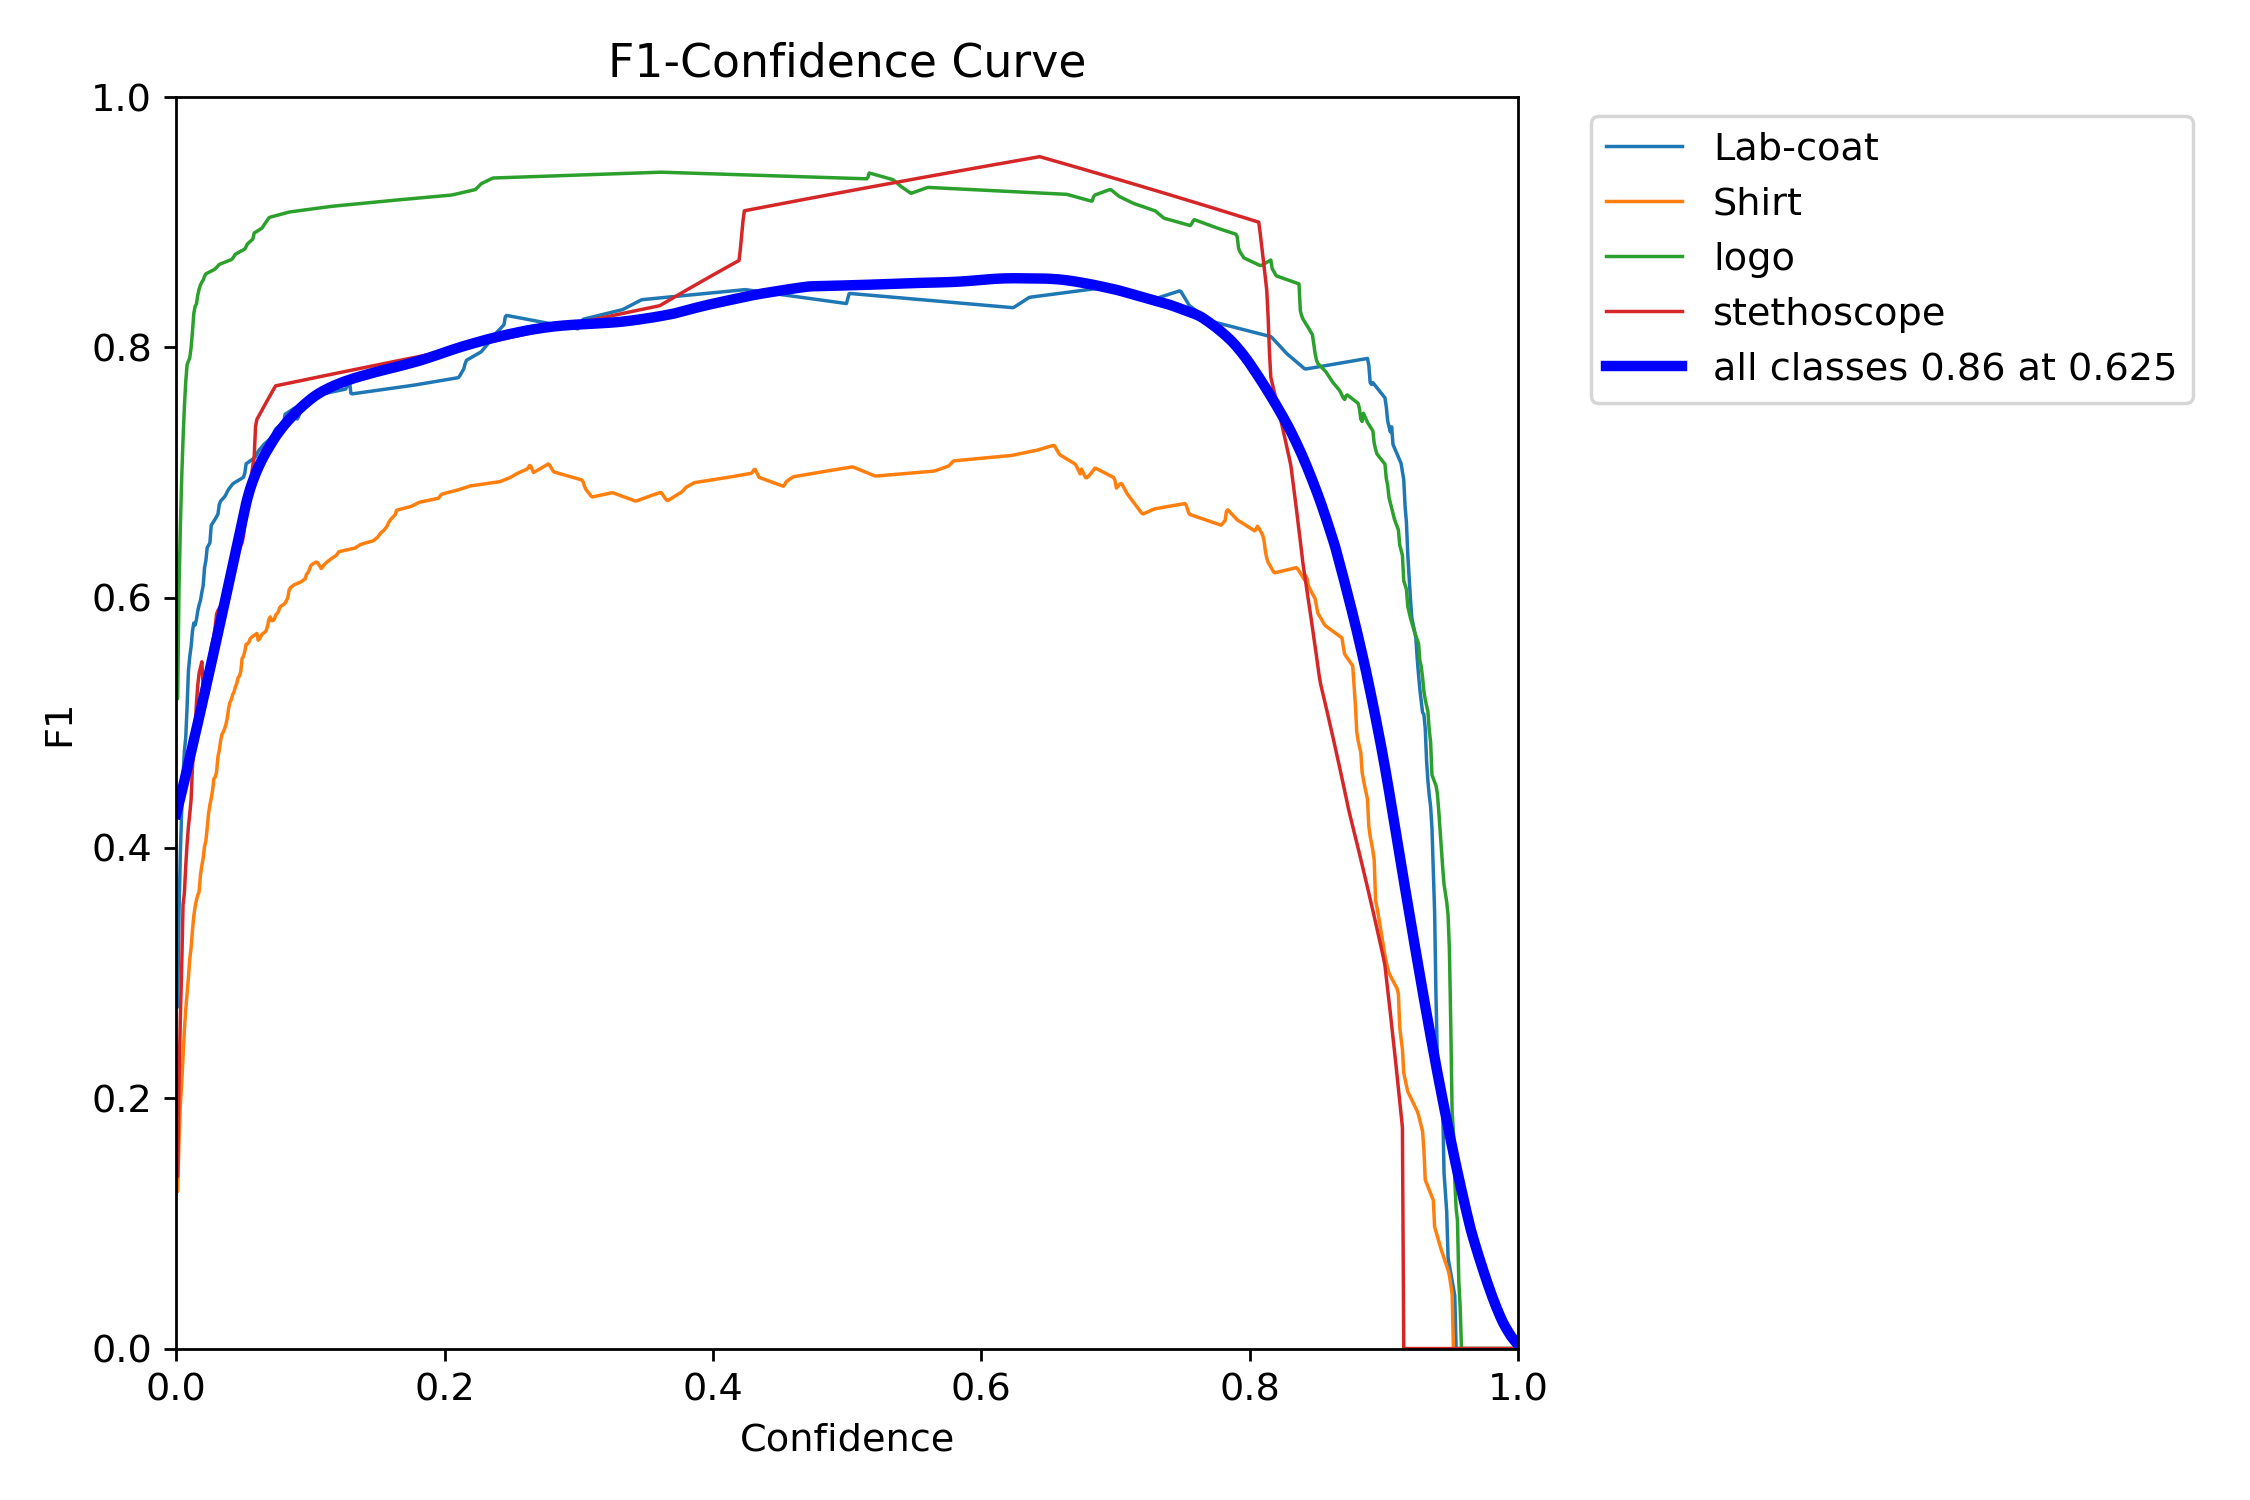
\includegraphics[width=\linewidth]{images/BoxF1_curve.png}
    \caption{Đường cong F1 theo confidence}
    \label{fig:yolo_box_f1_curve}
\end{subfigure}
\caption{Đường cong PR và F1 của YOLO11m trên tập test}
\label{fig:yolo_pr_f1_curves}
\end{figure}

\begin{figure}[H]
\centering
\begin{subfigure}{0.48\textwidth}
    \centering
    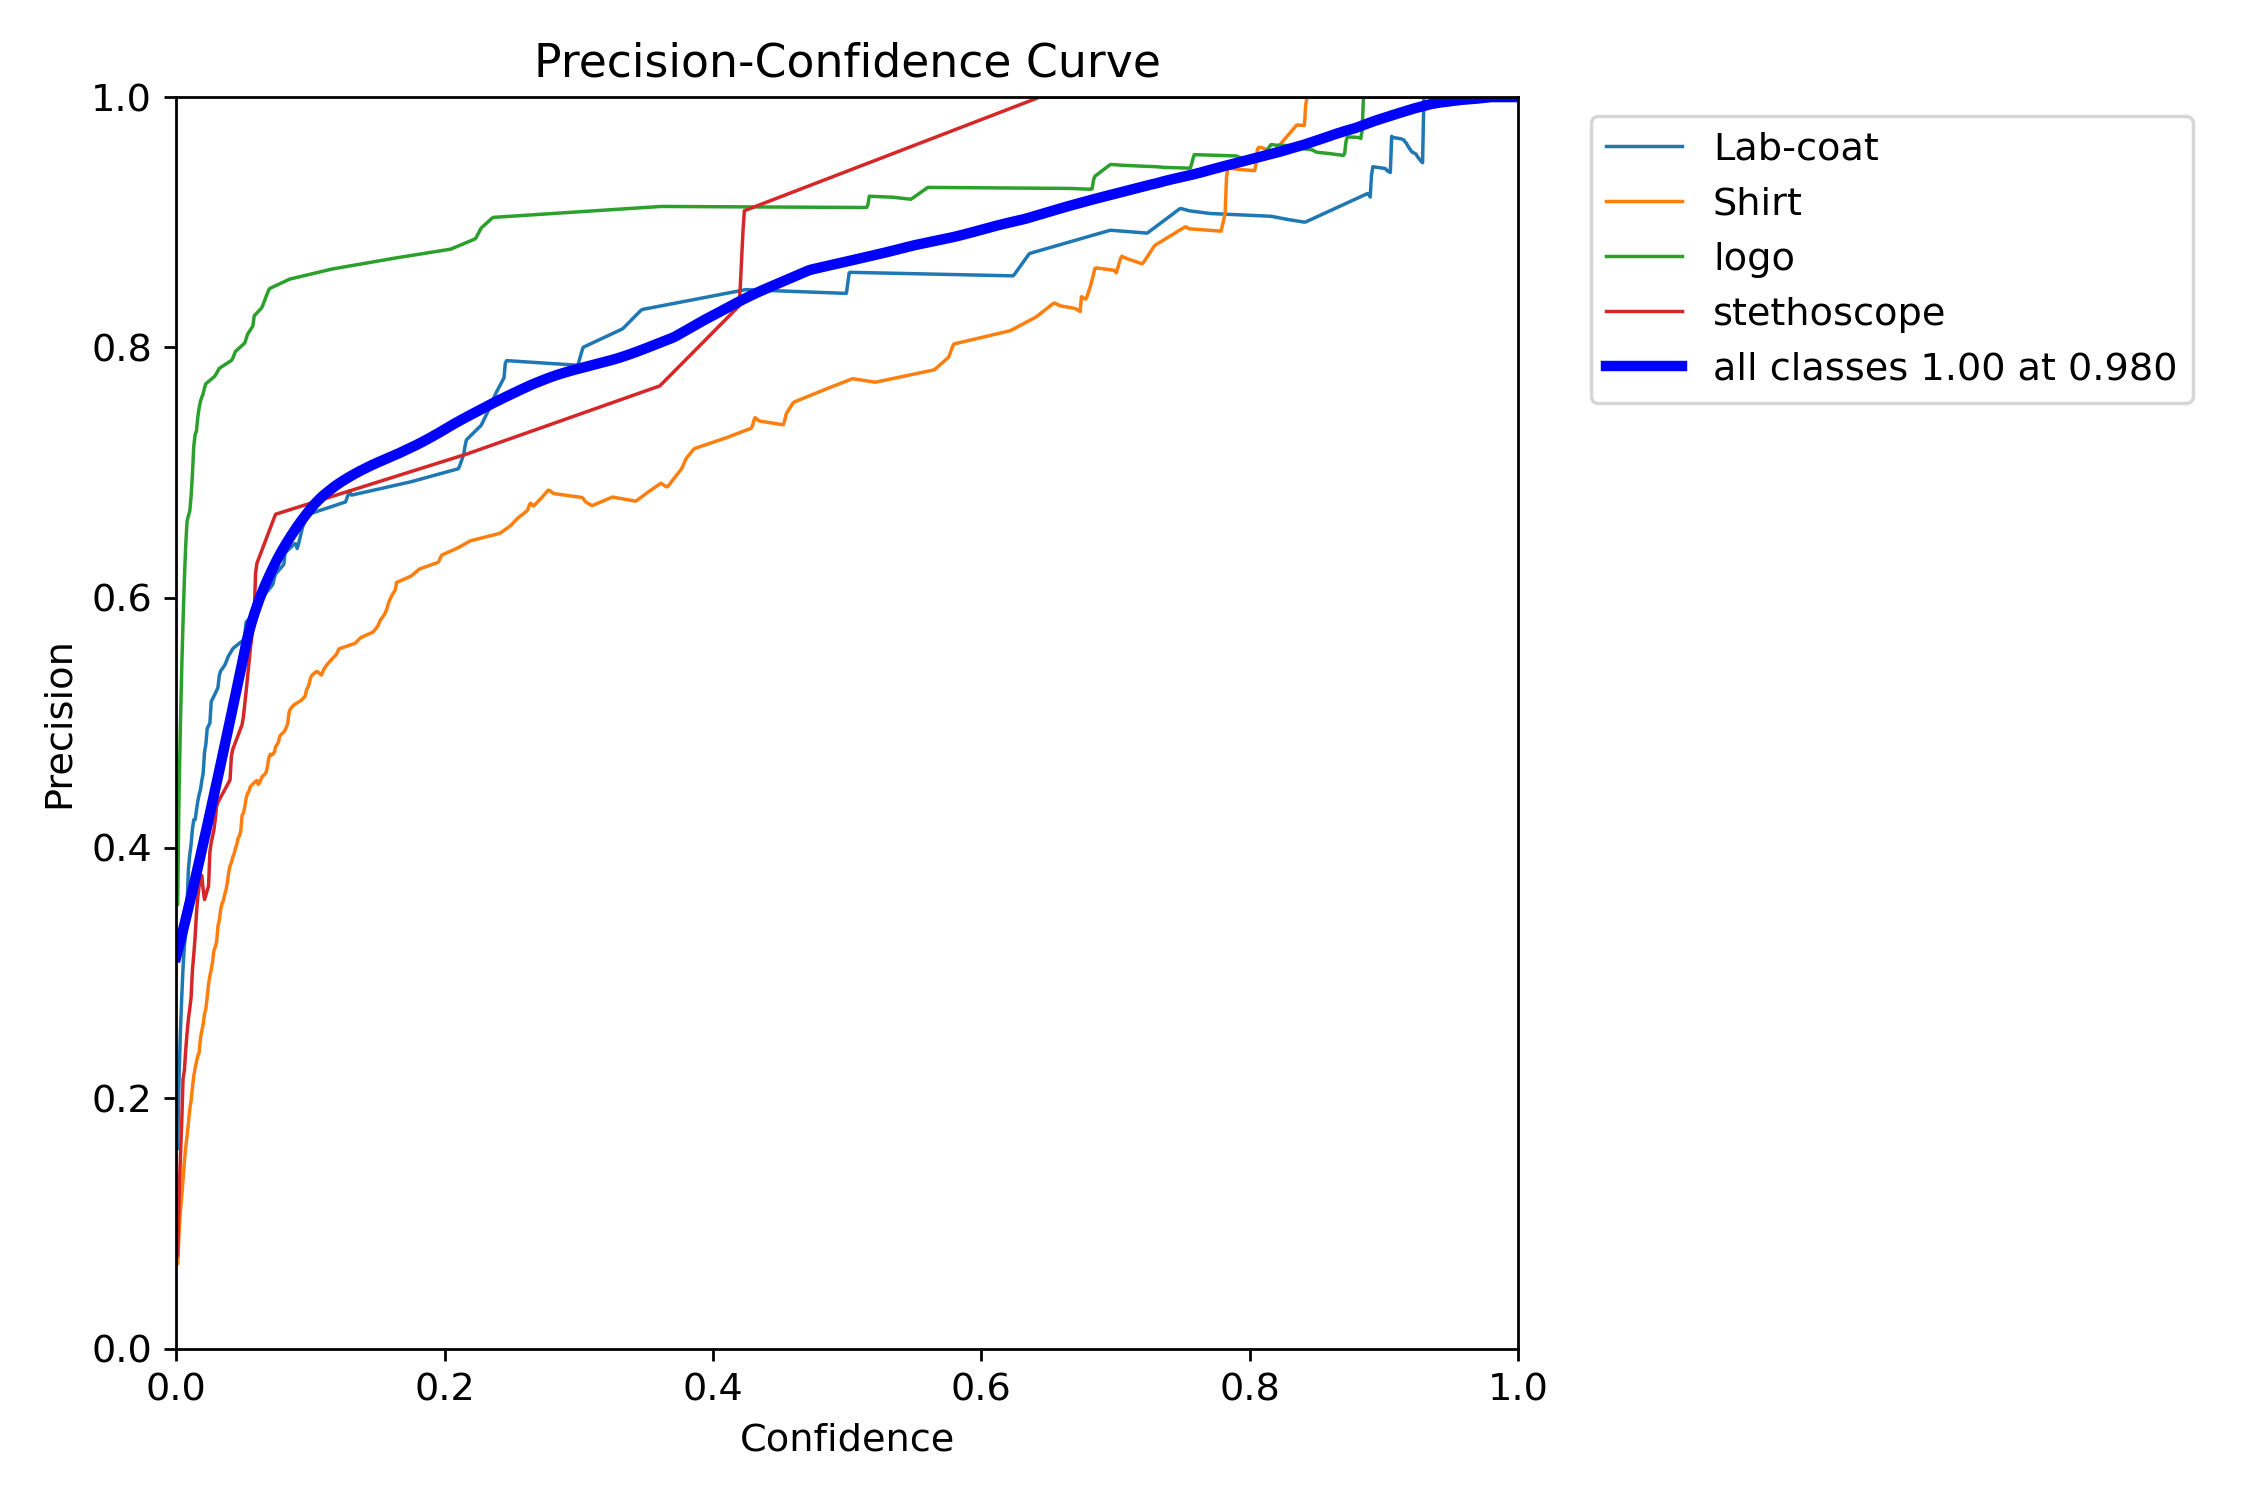
\includegraphics[width=\linewidth]{images/BoxP_curve.png}
    \caption{Precision theo confidence}
    \label{fig:yolo_box_p_curve}
\end{subfigure}
\hfill
\begin{subfigure}{0.48\textwidth}
    \centering
    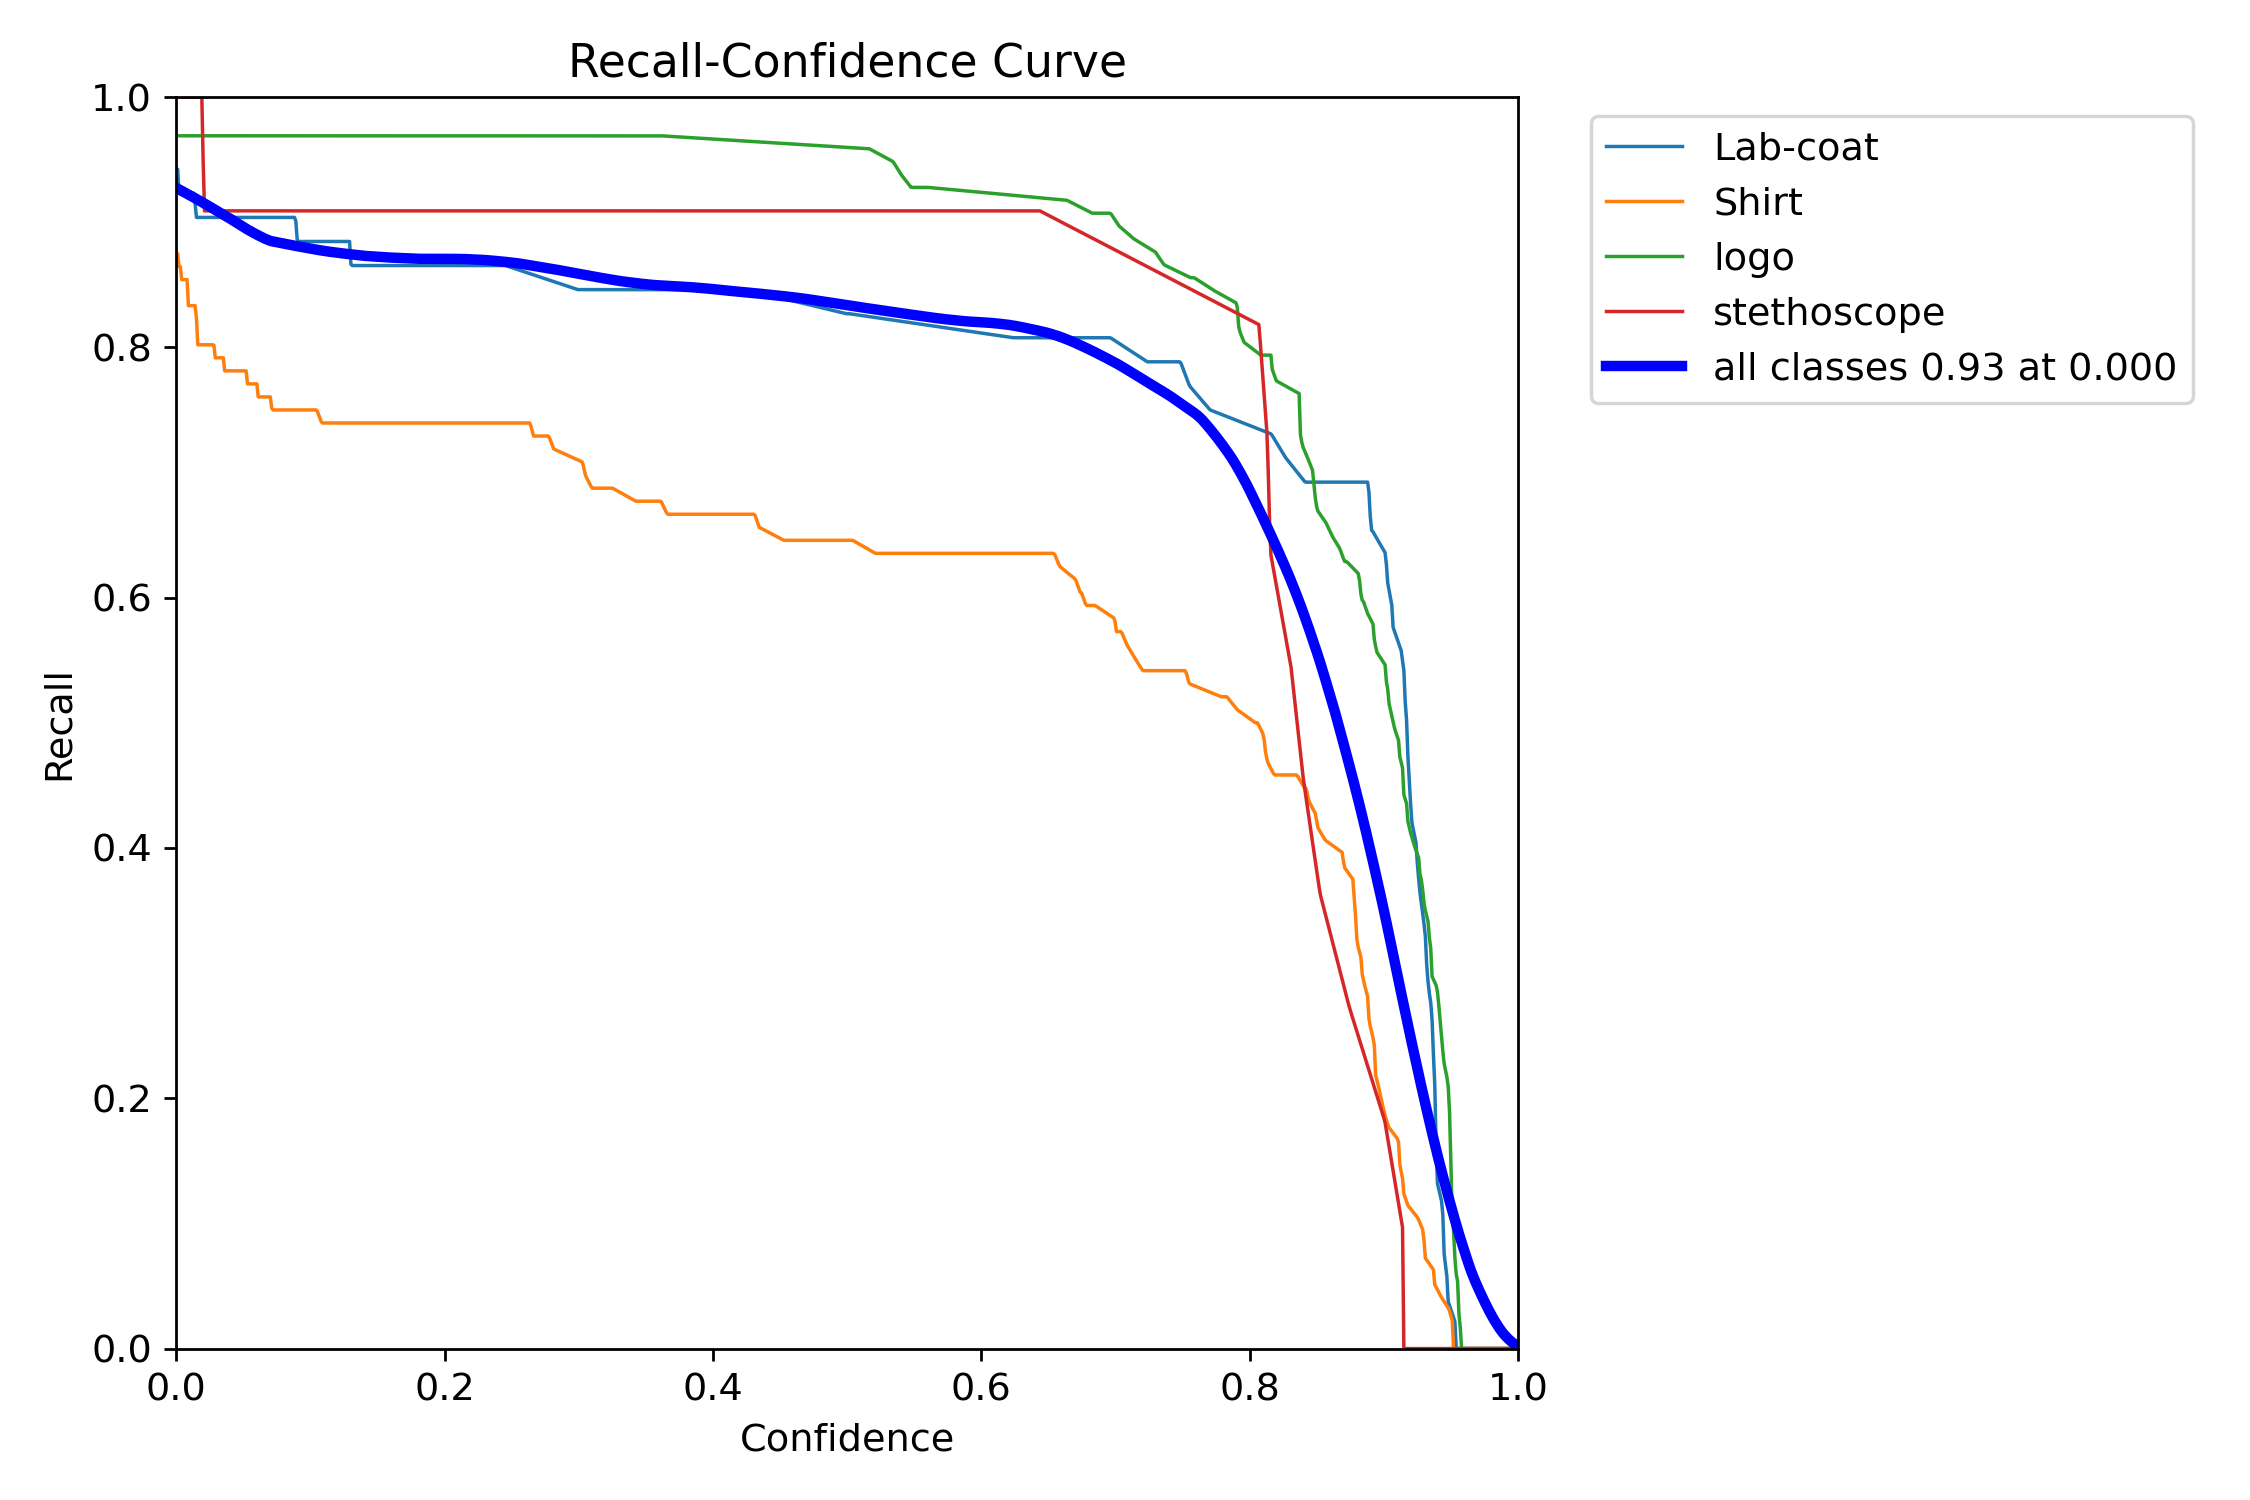
\includegraphics[width=\linewidth]{images/BoxR_curve.png}
    \caption{Recall theo confidence}
    \label{fig:yolo_box_r_curve}
\end{subfigure}
\caption{Đường cong Precision và Recall của YOLO11m trên tập test}
\label{fig:yolo_p_r_curves}
\end{figure}

Các đường cong trong Hình~\ref{fig:yolo_pr_f1_curves} và Hình~\ref{fig:yolo_p_r_curves} cho thấy sự đánh đổi giữa Precision và Recall khi thay đổi ngưỡng confidence. Trong hệ thống đề xuất, các hình này được dùng để hiểu hành vi kỹ thuật của nhánh YOLO và lựa chọn ngưỡng suy luận phù hợp; chúng không phải bằng chứng độc lập để kết luận một nội dung quảng cáo vi phạm pháp lý.

\subsection{Phân tích kết quả YOLO}
\texttt{logo} là lớp có kết quả tốt nhất với mAP50 = 0.948 và mAP50-95 = 0.835. Đây là tín hiệu quan trọng vì logo hoặc biểu tượng tổ chức có thể liên quan đến nhóm nguy cơ mạo danh hoặc lợi dụng uy tín. \texttt{Lab-coat} đạt mAP50 = 0.870 và mAP50-95 = 0.749, cho thấy mô hình nhận diện khá tốt hình ảnh áo blouse trắng.

\texttt{stethoscope} đạt Precision và Recall cao, nhưng chỉ có 11 instances trên test set. Vì vậy, kết quả của lớp này nên được xem là tín hiệu bước đầu, cần bổ sung thêm mẫu để đánh giá chắc chắn hơn. \texttt{Shirt} có Recall thấp hơn, nhưng đây là lớp phụ được thêm vào để giảm nhầm lẫn với \texttt{Lab-coat}; do đó không nên diễn giải \texttt{Shirt} như dấu hiệu rủi ro pháp lý độc lập.

\section{Thảo luận chung}
Kết quả thực nghiệm cho thấy hai nhánh PhoBERT và YOLO bổ sung cho nhau. PhoBERT phát hiện các tín hiệu ngôn ngữ như tuyên bố công dụng, tuyên bố chữa bệnh hoặc tham chiếu uy tín. YOLO phát hiện các dấu hiệu hình ảnh như áo blouse, logo và ống nghe. Khi được kết hợp trong tầng fusion, các tín hiệu này có thể giúp ưu tiên các mẫu quảng cáo cần rà soát kỹ hơn.

Tuy nhiên, cả hai nhánh đều có giới hạn riêng. PhoBERT gặp khó khăn với các nhãn hiếm và các cách diễn đạt gián tiếp. YOLO chỉ phát hiện đối tượng hình ảnh và không hiểu đầy đủ ngữ cảnh pháp lý. Vì vậy, kết quả cuối cùng cần được tổng hợp với OCR, ASR, rule-based detection và kiểm tra thủ công.

\section{Hạn chế và hướng cải thiện}
Các hạn chế chính gồm:
\begin{itemize}
    \item Test set hình ảnh hiện mới gồm 160 ảnh, cần mở rộng thêm để đánh giá chắc chắn hơn.
    \item Lớp \texttt{stethoscope} có số lượng mẫu ít nên kết quả có thể chưa đại diện đầy đủ.
    \item Dataset có cảnh báo lẫn giữa bounding box và segmentation annotation; trong quá trình đánh giá, Ultralytics chỉ sử dụng bounding box. Cần chuẩn hóa lại dataset ở version sau để tránh warning.
    \item Một số nhãn văn bản như \texttt{TESTIMONIAL} và \texttt{FEAR\_URGENCY} có support thấp, làm giảm macro F1.
    \item Cơ chế fusion hiện cần được hoàn thiện thêm để học hoặc hiệu chỉnh trọng số giữa các nhánh.
\end{itemize}

Trong các phiên bản tiếp theo, đề tài cần mở rộng dữ liệu thật, tăng số mẫu cho các lớp/nhãn hiếm, chuẩn hóa annotation hình ảnh, bổ sung đánh giá OCR/ASR và kiểm thử tầng fusion trên tập dữ liệu đa phương thức đã được review thủ công.
